% =========================================================================
% ASET 2026 — Closed-Loop LLM Task Planning for a Simulated Mobile
% Manipulator: An Implementation Study and Honest Reliability Analysis
%
% Build: pdflatex twice (cross-references). Requires IEEEtran, tikz,
% pgfplots and the figures/ folder.
% =========================================================================
\documentclass[conference]{IEEEtran}
\usepackage{cite}
\usepackage{amsmath,amssymb,amsfonts}
\usepackage{graphicx}
\graphicspath{{figures/}}
\usepackage{array}
\usepackage{booktabs}
\usepackage{textcomp}
\usepackage{xcolor}
\usepackage{url}
\usepackage{tikz}
\usetikzlibrary{arrows.meta,positioning,calc,backgrounds,fit}
\usepackage{pgfplots}
\pgfplotsset{compat=1.18}

% ── Design tokens (validated categorical palette; blue=LLM, orange=baseline) ──
\definecolor{llmblue}{HTML}{2A78D6}
\definecolor{llmbluefill}{HTML}{DCEAFB}
\definecolor{baseorange}{HTML}{EB6834}
\definecolor{baseorangefill}{HTML}{FBE2D6}
\definecolor{inkprimary}{HTML}{0B0B0B}
\definecolor{inksecondary}{HTML}{52514E}
\definecolor{gridgray}{HTML}{E6E6E3}
\definecolor{panelgray}{HTML}{F4F4F2}

\begin{document}

\title{Closed-Loop Large Language Model Task Planning for a Simulated
Mobile Manipulator:\\ An Implementation Study and Honest Reliability Analysis}

\author{%
\begin{minipage}{\textwidth}\centering
  \begin{minipage}[t]{0.31\textwidth}\centering
    Firaol Tesfaye\\
    Higher Colleges of Technology\\
    Dubai, UAE\\
    h00539876@hct.ac.ae
  \end{minipage}\hfill
  \begin{minipage}[t]{0.31\textwidth}\centering
    Milki Teshome\\
    Higher Colleges of Technology\\
    Dubai, UAE\\
    h00539899@hct.ac.ae
  \end{minipage}\hfill
  \begin{minipage}[t]{0.31\textwidth}\centering
    Yassine Benachour\\
    Higher Colleges of Technology\\
    Dubai, UAE\\
    ybenachour@hct.ac.ae
  \end{minipage}\\[1.3em]
  \begin{minipage}[t]{0.31\textwidth}\centering
    Ammar Natsheh\\
    Higher Colleges of Technology\\
    Dubai, UAE\\
    anatsheh@hct.ac.ae
  \end{minipage}
\end{minipage}}

\maketitle

% =========================================================================
\begin{abstract}
We present a reproducible closed-loop large language model (LLM) task
planner for a mobile manipulator, built on an open-source stack (ROS~2,
Gazebo, Nav2, MoveIt~2). The LLM receives a natural-language command and a
structured scene state and acts only by calling typed robot tool services;
a fresh scene state after every action closes the perception--action loop
and enables autonomous replanning after execution failures. We compare this
planner against a hardcoded baseline that runs the same task through the
same tool server and grasp implementation with a fixed, perception-blind
sequence and no recovery.
Single-object pick-and-deliver is reported complete in 13/16 trials, most
of them involving an autonomous recovery from a failed first grasp. Outcomes
were self-reported rather than checked against the simulator, and four of
those runs end with a failed or timed-out place, so the true rate lies
between 9/16 and 13/16. The baseline is faster and repeatable on its tuned
configuration but cannot adapt, and LLM reliability degrades on
multi-object and ambiguous commands.
We report all outcomes, including residual failure modes, and distill
integration lessons for practitioners building similar systems.
\end{abstract}

\begin{IEEEkeywords}
large language models, task planning, mobile manipulation, ROS~2,
closed-loop control, human--robot instruction
\end{IEEEkeywords}

% =========================================================================
\section{Introduction}

Instructing a robot in natural language---\emph{``take the red cube to
dispatch''}---and having it decompose the task, execute it, and recover
from failures without task-specific scripting is a long-standing goal of
service and warehouse robotics. Traditional industrial automation achieves
reliability through exhaustive pre-programming: every contingency is
anticipated and hardcoded by an engineer, and the resulting system is fast
and repeatable precisely as long as the world matches its program. The cost
is rigidity. A change as simple as \emph{``prioritize the red boxes
today''} requires re-engineering, not a sentence.

Large language models (LLMs) have recently made the language-understanding
and task-decomposition steps tractable~\cite{saycan,codeaspolicies}. A
language model alone, however, cannot move a robot: it must be grounded in
a real perception--action stack, and---critically---it must \emph{react}
when the physical world does not match its plan. Much of the published
work in this space demonstrates open-loop planning, in which the model
emits a plan once and the robot executes it blindly; comparatively little
reports, quantitatively, what happens when a general-purpose LLM is wired
into a conventional robotics stack as a persistent closed-loop decision
maker.

This paper is an \emph{implementation study}. Rather than proposing a new
planning algorithm, we ask a practical question: how far does an
off-the-shelf, general-purpose LLM, constrained to a fixed tool-calling
interface and closed with structured scene-state feedback, actually get on
a mobile-manipulation task---and where does it fail? We build
the complete system (Section~\ref{sec:architecture}), define a hardcoded
baseline that isolates decision-making from raw capability
(Section~\ref{sec:baseline}), and evaluate both on single-object,
multi-object, and ambiguous-command scenarios
(Section~\ref{sec:results}).

Our contributions are:
\begin{enumerate}
    \item a reproducible closed-loop LLM mobile-manipulation system on a
    fully open-source stack, with the LLM confined to a typed tool
    interface and per-action scene-state feedback;
    \item a comparison against a hardcoded baseline sharing the same tool
    server and grasp implementation, which isolates decision-making from
    stack capability but
    is not a controlled test of adaptivity, since the baseline is
    non-reactive by construction; and
    \item a transparent reliability analysis: success rates with confidence
    intervals, a failure-mode catalogue, and integration lessons.
\end{enumerate}

% =========================================================================
\section{Related Work}
\label{sec:related}

\textbf{LLMs as robot task planners.} SayCan~\cite{saycan} grounds an LLM
in a library of robot skills scored by learned affordances; Code as
Policies~\cite{codeaspolicies} has the LLM emit executable policy code, and
ProgPrompt~\cite{progprompt} showed structured prompting improves plan
validity. End-to-end vision-language-action models such as
PaLM-E~\cite{palme} and RT-2~\cite{rt2}, and value-map composition as in
VoxPoser~\cite{voxposer}, form a parallel line; a recent survey catalogues
the space~\cite{llmrobosurvey}. We instead follow the \emph{tool-calling}
paradigm native to commercial LLM APIs---akin to ReAct~\cite{react} and
Toolformer~\cite{toolformer}: the model only calls typed ROS~2 services
with schema-validated arguments, which bounds the action space and makes
every decision auditable.

\textbf{Closing the loop.} Inner Monologue~\cite{innermonologue} showed
that feeding textual environment feedback back into the LLM materially
improves long-horizon performance. We adopt this principle end-to-end: a
structured scene state is appended to the conversation after \emph{every}
action, so the planner reasons over current reality rather than stale
assumptions. Vemprala~et~al.~\cite{chatgptrobotics} report similar design
principles for ChatGPT-driven robotics, largely through demonstrations.

\textbf{Position of this work.} We claim no algorithmic novelty over these
paradigms; we contribute a fully open-stack, end-to-end implementation, a
baseline sharing the same tool server and grasp implementation
(Section~\ref{sec:baseline}), and a candid reliability analysis
that---like SayCan's failure appendices---treats characterized failure
modes as a result rather than an embarrassment. The stack components are
documented in their systems papers: ROS~2~\cite{ros2}, Nav2~\cite{nav2},
MoveIt~\cite{moveit}, and YOLOv8~\cite{yolov8}.

% =========================================================================
\section{System Architecture}
\label{sec:architecture}

% FIGURE 1 -----------------------------------------------------------------
\begin{figure}[t]
\centering
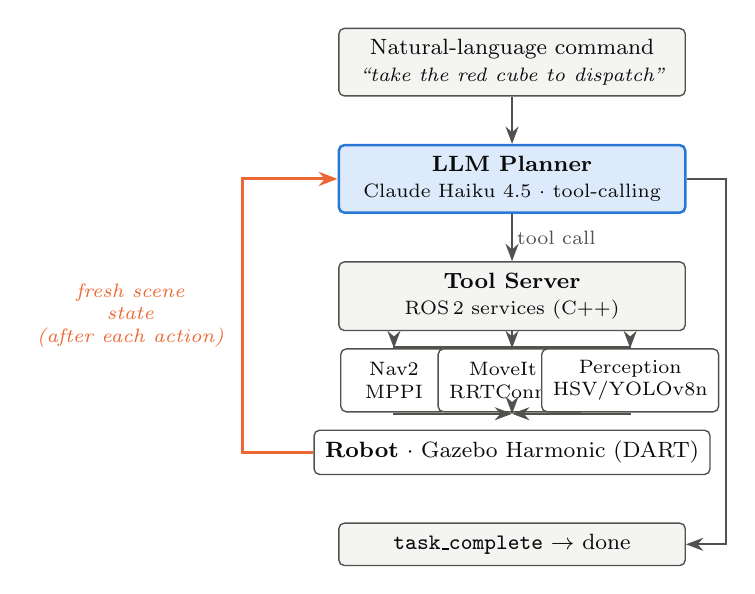
\begin{tikzpicture}[
    font=\footnotesize,
    node distance=6mm,
    box/.style={rounded corners=2pt, draw=inksecondary, line width=0.5pt,
                align=center, inner sep=4pt, text=inkprimary},
    io/.style={box, fill=panelgray, minimum width=44mm},
    llm/.style={box, fill=llmbluefill, draw=llmblue, line width=0.9pt,
                minimum width=44mm},
    tool/.style={box, fill=panelgray, minimum width=44mm},
    comp/.style={box, fill=white, minimum width=13.5mm, minimum height=8mm,
                 font=\scriptsize},
    robot/.style={box, fill=white, minimum width=44mm},
    flow/.style={-{Stealth[length=2.2mm]}, line width=0.7pt, draw=inksecondary},
    fb/.style={-{Stealth[length=2.4mm]}, line width=1.1pt, draw=baseorange},
    lbl/.style={font=\scriptsize, text=inksecondary, inner sep=1.5pt},
    fblbl/.style={font=\scriptsize\itshape, text=baseorange, align=center},
  ]
  \node[io] (cmd) {Natural-language command\\{\scriptsize\itshape ``take the red cube to dispatch''}};
  \node[llm, below=of cmd] (llm) {\textbf{LLM Planner}\\{\scriptsize Claude Haiku 4.5 $\cdot$ tool-calling}};
  \node[tool, below=of llm] (ts) {\textbf{Tool Server}\\{\scriptsize ROS\,2 services (C++)}};
  \node[below=5mm of ts] (compmid) {};
  \node[comp] (nav) at ($(compmid)+(-15mm,0)$) {Nav2\\{\scriptsize MPPI}};
  \node[comp] (moveit) at (compmid) {MoveIt~2\\{\scriptsize RRTConnect}};
  \node[comp] (perc) at ($(compmid)+(15mm,0)$) {Perception\\{\scriptsize HSV/YOLOv8n}};
  \node[robot, below=5mm of compmid] (robot) {\textbf{Robot} $\cdot$ Gazebo Harmonic (DART)};
  \node[io, below=of robot] (done) {\texttt{task\_complete} $\rightarrow$ done};

  % forward flow
  \draw[flow] (cmd) -- (llm);
  \draw[flow] (llm) -- node[lbl,right] {tool call} (ts);
  \draw[flow] (ts.south) -- ($(ts.south)+(0,-2mm)$) -| (nav.north);
  \draw[flow] (ts.south) -- ($(ts.south)+(0,-2mm)$) -| (moveit.north);
  \draw[flow] (ts.south) -- ($(ts.south)+(0,-2mm)$) -| (perc.north);
  \draw[flow] (nav.south) |- ($(robot.north)+(0,2mm)$);
  \draw[flow] (moveit.south) -- ($(robot.north)+(0,2mm)$);
  \draw[flow] (perc.south) |- ($(robot.north)+(0,2mm)$);
  \draw[flow] (llm.east) -- ++(5mm,0) |- (done.east);

  % feedback loop (the point of the paper) — up the left side
  \draw[fb] (robot.west) -- ++(-9mm,0)
        |- node[fblbl,pos=0.25,left=1mm] {fresh scene\\state\\{\scriptsize(after each action)}} (llm.west);
\end{tikzpicture}
\caption{Closed-loop LLM task-planning architecture. The planner acts only
through typed tool services; after \emph{every} action a fresh structured
scene state (orange) is returned to the model, enabling replanning on
failure. The loop runs until \texttt{task\_complete}.}
\label{fig:architecture}
\end{figure}

\subsection{Platform}

The robot is a differential-drive base carrying a custom 6-DOF arm (six
revolute joints, each limited to $\pm3.14$\,rad), a two-finger gripper with
a mimic-coupled passive finger, and an RGB-D camera. The arm was designed
in SolidWorks and exported to URDF; the export required non-trivial
correction (Section~\ref{sec:lessons}), including a PCA plane fit on the
base-plate mesh to remove an $8.1^{\circ}$ tilt baked into the CAD
assembly frame.

The robot is simulated in Gazebo Sim 8.11 (Harmonic) with the DART physics
engine under ROS~2 Jazzy on Ubuntu 24.04. Navigation uses Nav2 with the
MPPI controller against a frozen static map (an identity
$map \rightarrow odom$ transform with a pre-built occupancy grid; no live
SLAM runs during experiments, for reasons detailed in
Section~\ref{sec:lessons}). Arm motion uses MoveIt~2
(\texttt{MoveGroupInterface}) with the OMPL RRTConnect planner. Object
detection uses HSV color segmentation (the primary and default detector,
used in all reported experiments), with an optional Ultralytics
YOLOv8n~\cite{yolov8} mode selectable by parameter; detections are back-projected through the
depth image and camera intrinsics and transformed to the map frame via TF2.
Grasping is modeled with a kinematic attachment constraint (Gazebo's
DetachableJoint): upon gripper closure, a rigid joint is created between
the gripper link and the target object, \emph{conditioned on the
end-effector being within a proximity threshold of the object}. This
abstracts low-level contact dynamics---a common simplification in
simulation-based manipulation research---while preserving meaningful grasp
success/failure outcomes determined by whether the arm actually reaches the
target.

The software is organized into seven ROS~2 packages. All nodes are C++
(\texttt{rclcpp}) except exactly two Python (\texttt{rclpy}) nodes---the
perception node and the LLM client---reflecting the practical reality
that ML tooling lives in Python while the control and service layer
benefits from C++.

% FIGURE 2 -----------------------------------------------------------------
\begin{figure}[t]
\centering
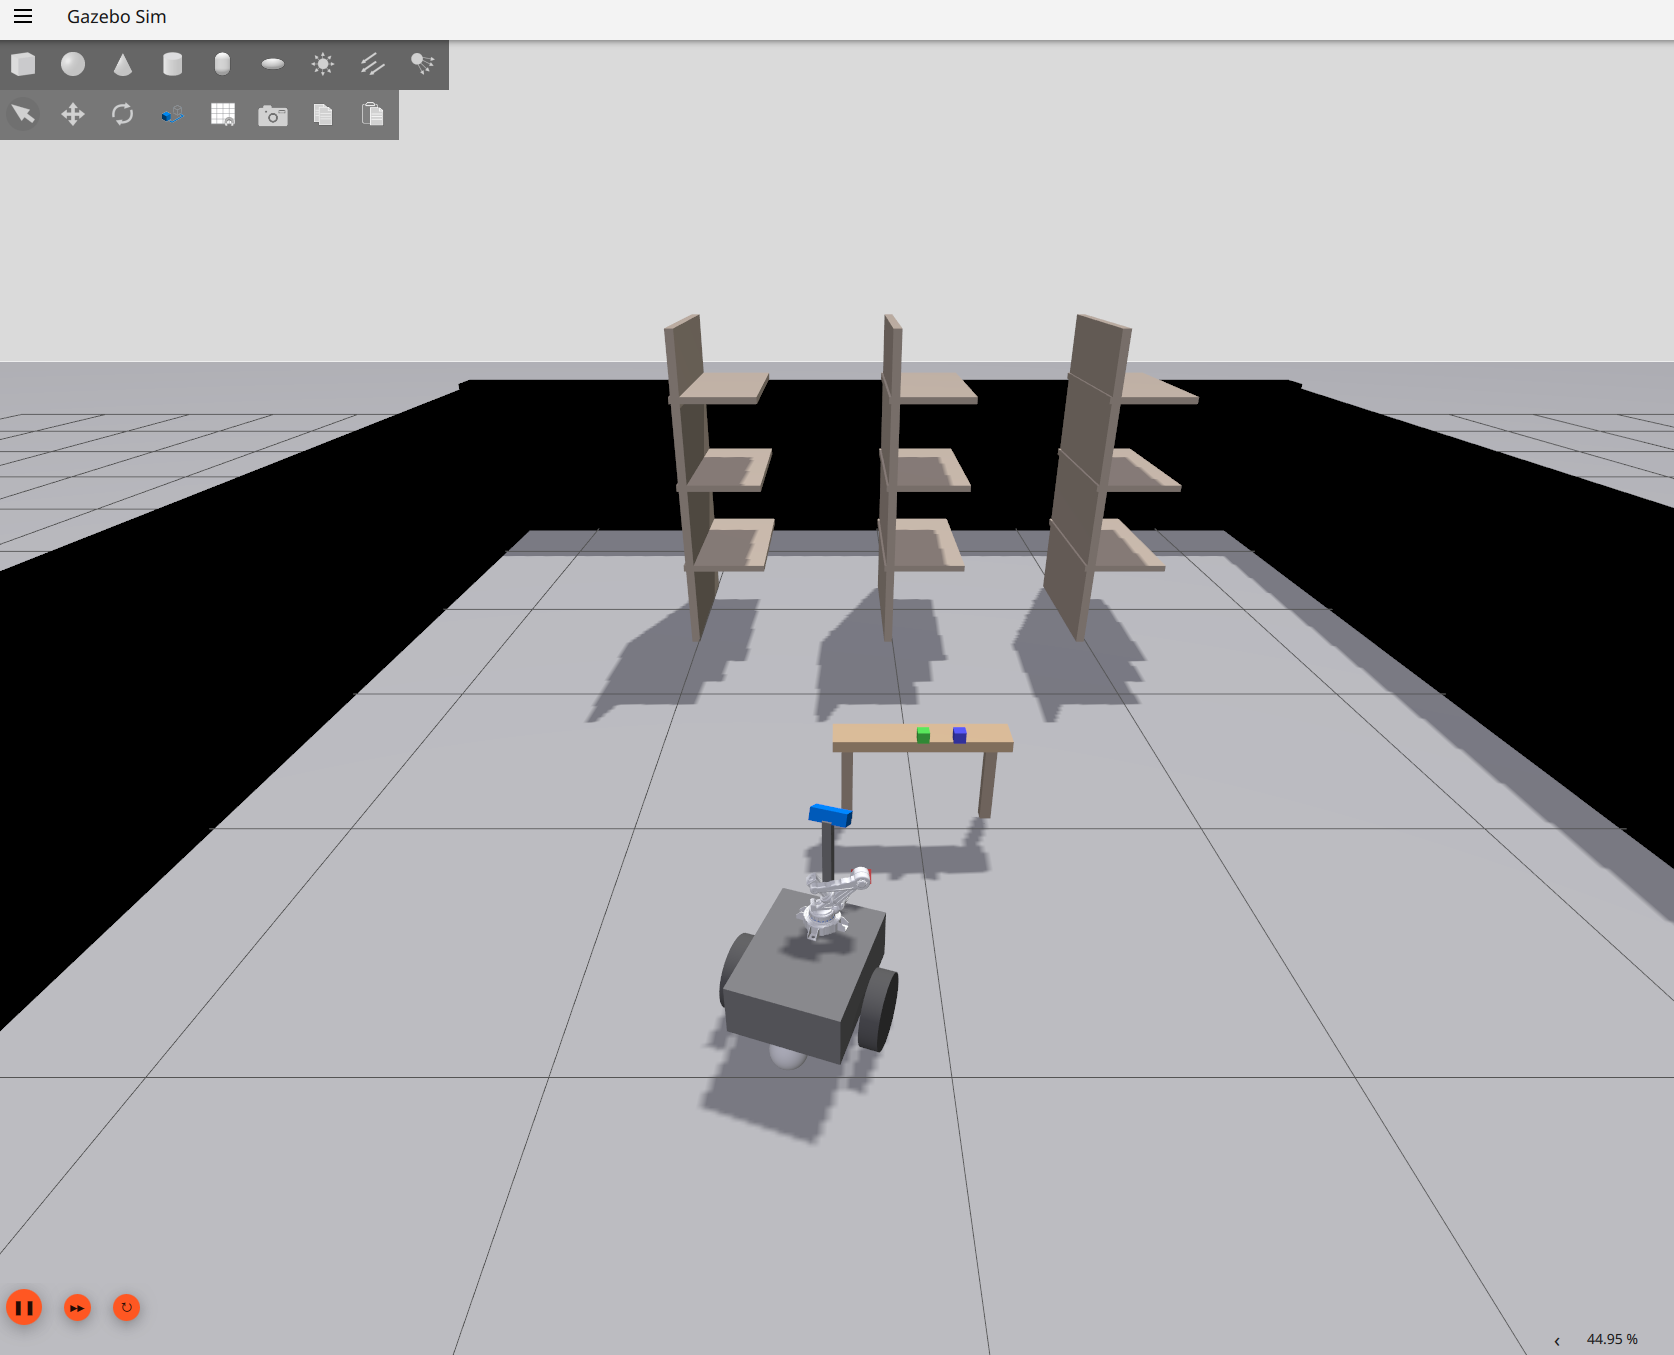
\includegraphics[width=\columnwidth]{fig_world.png}
\caption{Simulated warehouse environment and the mobile manipulator
platform: the differential-drive base with its 6-DOF arm and camera mast,
the pick table with colored cubes, and the storage shelves.}
\label{fig:world}
\end{figure}

\subsection{Tool Server}

A C++ tool server exposes the robot's capabilities as ROS~2 services, each
a self-contained, blocking, verifiable action returning
\texttt{\{success, message\}}. The eleven tools available to the planner
are: \texttt{navigate\_to}, \texttt{drive\_distance},
\texttt{detect\_objects}, \texttt{move\_arm\_to\_named} (home/ready),
\texttt{move\_arm\_to\_pose}, \texttt{pick}, \texttt{place},
\texttt{open\_gripper}, \texttt{close\_gripper}, \texttt{get\_state}, and
\texttt{task\_complete}. \texttt{navigate\_to} drives Nav2 to one of four
named locations (\texttt{table}, \texttt{dispatch\_zone},
\texttt{shelf\_area}, \texttt{home}); \texttt{drive\_distance} performs a
short, blind dead-reckoning move (capped at $\pm2$\,m) for local
adjustments; \texttt{pick} performs a perception-driven grasp: it looks up
the target's detected 3-D position, plans a pre-grasp pose above it,
descends, verifies proximity, and only then closes the gripper and triggers
the attachment---so a pick attempted out of reach \emph{fails}, and that
failure is reported back to the planner. Every tool call, result, and
duration is logged. Table~\ref{tab:tools} specifies each tool's arguments,
output, success condition, and representative failure message.

\begin{table*}[t]
\caption{Robot Tool Interface Exposed to the LLM Planner. Every tool returns
\texttt{\{success:\,bool, message:\,string\}}; the planner acts only through
these typed services. Two further tools make no robot call:
\texttt{get\_state} returns the scene state (auto-appended after every
action) and \texttt{task\_complete(success, summary)} ends the loop.}
\label{tab:tools}
\centering
\scriptsize
\setlength{\tabcolsep}{4pt}
\begin{tabular}{@{}>{\raggedright\arraybackslash}p{3.4cm}>{\raggedright\arraybackslash}p{3.4cm}>{\raggedright\arraybackslash}p{4.6cm}>{\raggedright\arraybackslash}p{4.8cm}@{}}
\toprule
\textbf{Tool} & \textbf{Arguments} & \textbf{Success condition} & \textbf{Representative failure message} \\
\midrule
\texttt{navigate\_to} & \texttt{location} $\in$ \{table, dispatch\_zone, shelf\_area, home\} & Nav2 reaches the goal within tolerance (0.25\,m / 0.15\,rad) & ``Navigation failed'' (timeout / unreachable) \\
\texttt{drive\_distance} & \texttt{distance\_m} ($\pm2$\,m cap) & Dead-reckoned displacement completed & ``Distance exceeds 2\,m safety cap'' \\
\texttt{detect\_objects} & --- & Detector returns $\geq1$ detection & ``No detections available'' \\
\texttt{move\_arm\_to\_named} / \texttt{\_pose} & \texttt{pose} $\in$ \{home, ready\} / Cartesian target & MoveIt plans and executes to the target & ``Failed to reach ready staging pose'' / ``Pose move failed'' \\
\texttt{pick} & \texttt{object\_label} & Pre-grasp IK solved, descent + attach within proximity (0.08\,m) & ``$X$ is out of reach (pre-grasp IK failed)'' \\
\texttt{place} & \texttt{location} & Held object released at target & ``No object currently held'' \\
\texttt{open\_gripper} / \texttt{close\_gripper} & --- & Gripper joints reach commanded state & ``Gripper command timed out'' \\
\bottomrule
\end{tabular}
\end{table*}

\subsection{Closed-Loop LLM Planner}

The planner (Fig.~\ref{fig:architecture}) exposes a ROS~2 action
\texttt{/execute\_task}. Given a command, it fetches an initial scene
state, starts an LLM conversation governed by a fixed system prompt, and
loops for up to \texttt{max\_turns} tool-result rounds (25 or 30 depending
on scenario; Table~\ref{tab:llmconfig}). We report \emph{model calls}
rather than turns: the opening call that receives the command precedes the
first round, so a run that exhausts a 25-turn budget makes 26 calls. At
each turn the
model either requests a tool call---dispatched generically by constructing
the service request from the tool's schema and polling the result with a
200\,s deadline---or calls \texttt{task\_complete}. Crucially, after every
\texttt{navigate\_to}, \texttt{drive\_distance}, \texttt{pick}, or
\texttt{place}, a fresh structured scene state is appended to the
conversation, giving the model up-to-date robot pose and detected-object
coordinates before its next decision. Repeated identical failures trigger
an injected corrective hint to break loops. Every turn, tool call, timing,
and the full conversation are logged to JSON for analysis. The evaluated
model is Anthropic Claude Haiku 4.5, selected as a fast, low-cost model
representative of what a practitioner would deploy in a high-frequency
replanning loop. Table~\ref{tab:llmconfig} reports the exact model and
decoding configuration used in all reported runs.

The planner has \emph{no automatic retry}: a failed tool call is not
re-issued by the harness. Instead, the failure message is appended to the
conversation and the model decides the next action---so every recovery is a
genuine LLM re-plan, not a scripted retry. The only harness intervention is
a loop-breaker: if the identical \texttt{(tool, arguments, error)} signature
recurs twice in succession, a corrective hint is injected into the tool
result. Because the Anthropic Messages API is stateless, the full
conversation (system prompt, tool schemas, and growing scene-state history)
is re-sent on every turn; prompt caching was not enabled, so the reported
token counts and cost reflect the full uncached input.

\begin{table}[t]
\caption{LLM Planner Configuration (identical across all reported runs).}
\label{tab:llmconfig}
\centering
\footnotesize
\setlength{\tabcolsep}{3pt}
\begin{tabular}{@{}>{\raggedright\arraybackslash}p{2.7cm}>{\raggedright\arraybackslash}p{4.9cm}@{}}
\toprule
\textbf{Parameter} & \textbf{Value} \\
\midrule
Provider / SDK & Anthropic Messages API (\texttt{anthropic}~0.109) \\
Model & \texttt{claude-haiku-4-5-}\allowbreak\texttt{20251001} \\
Temperature & unset (provider default, 1.0) \\
\texttt{max\_tokens} (per call) & 1024 \\
Tool interface & native tool use, \texttt{tool\_choice}: auto \\
\texttt{max\_turns} & 25 (single-object) / 30 (multi-object, ambiguous) \\
Per-tool timeout & 200\,s \\
Retry policy & none (re-plan by re-prompting on failure) \\
Loop breaker & hint injected after 2 identical failures \\
Prompt caching & disabled (full history re-sent per turn) \\
System prompt & fixed plain-text file, unchanged across runs \\
\bottomrule
\end{tabular}
\end{table}

\subsection{The Single Most Important Reliability Margin}
\label{sec:margin}

The base navigates to a standoff in front of the table that leaves the
cubes at the very edge of the arm's reachable workspace; the first pick
from that pose therefore typically fails with a pre-grasp IK error. A short
forward \texttt{drive\_distance}(0.30\,m) ``approach nudge'' brings the
cube into reach. Whether this nudge is issued is the dominant factor in
single-object success---and it is \emph{not} hardcoded into the LLM's
path. The model must infer it from the failure message returned by the
tool server. As Section~\ref{sec:results} shows, it reliably does, and
this recovery is the clearest demonstration of the closed loop working as
designed.

% =========================================================================
\section{Baseline Controller}
\label{sec:baseline}

To isolate the contribution of closed-loop LLM decision-making from the
raw capability of the stack, the baseline executes the same task through
the \emph{same} tool server, differing only in how the next action is
chosen. It runs a fixed sequence---\texttt{navigate\_to(table)}
$\rightarrow$ \texttt{drive\_distance(0.30)} $\rightarrow$
\texttt{pick\_at\_pose} $\rightarrow$
\texttt{navigate\_to(dispatch\_zone)} $\rightarrow$
\texttt{place}---with three deliberate properties of a traditional
automation program: (i) it picks at a compile-time-constant coordinate and
never calls perception; (ii) it does not branch on scene state; and
(iii) it has no recovery---any failed step aborts the run. A two-cube mode
repeats the sequence for a second object. \texttt{pick\_at\_pose} is the one
service the baseline uses that the planner does not: the planner's
\texttt{pick} takes an object label and resolves its position from live
perception at call time (Table~\ref{tab:tools}), whereas
\texttt{pick\_at\_pose} takes a literal coordinate, synthesises a detection
at it, and delegates to the same grasp routine. The two systems therefore
share the grasp implementation and differ only in where the target position
comes from. The baseline is thus fast,
deterministic, and rigid by construction: it embodies the ``sophisticated
flowchart'' character of conventional warehouse automation that motivated
this study.

% =========================================================================
\section{Experimental Setup}
\label{sec:setup}

An automated experiment runner resets the world before each trial (release
and open the gripper, return the arm home, restore cube spawn poses,
return the base to its home pose), then issues the command and records
success, wall-clock duration, path length, and---for the LLM---the number
of model calls and failed tool calls. Path length is recorded in the
released logs but is not analysed in this paper. The simulated warehouse and robot
platform are shown in Fig.~\ref{fig:world}. A trial is scored a
\emph{success} when the system under test reports the delivery complete---
\texttt{task\_complete(success=true)} for the planner, a successful final
step for the baseline---and a \emph{failure} if the run aborts, exceeds the
turn limit (Table~\ref{tab:llmconfig}), or the planner calls
\texttt{task\_complete(success=false)}. A per-tool 200\,s timeout is logged
and returned to the planner as a failed tool call, but does not itself end
the trial: the planner may keep acting and still report completion, which is
why some counted successes contain a timed-out call
(Section~\ref{sec:verif}). For the baseline, which has no recovery path, a
timed-out step does abort the run. This criterion is self-reported and was
not checked against the simulator;
Section~\ref{sec:verif} quantifies what that costs and describes the
ground-truth check now in the release; Section~\ref{sec:provenance} states
which log produced each reported number. Table~\ref{tab:scenarios}
details the scenarios, their initial conditions, and stopping criteria.

\begin{table*}[t]
\caption{Evaluation Scenarios: Initial Conditions, Trial Count, and Stopping Criteria.}
\label{tab:scenarios}
\centering
\small
\begin{tabular}{@{}llp{3.4cm}cp{2.6cm}p{3.4cm}@{}}
\toprule
\textbf{ID} & \textbf{System} & \textbf{Command / initial condition} & \textbf{$N$} & \textbf{Success criterion} & \textbf{Failure / limit} \\
\midrule
S1 & LLM & ``take the red cube to dispatch''; red cube on table & 5 & red cube in dispatch zone & abort or turn limit \\
S2 & LLM & ``bring the red cube to dispatch''; all three cubes on table & 7 & the \emph{red} cube in dispatch zone & abort or turn limit \\
S4 & LLM & as S1, cube displaced $\approx$18\,cm 5\,s after departure & 4 & red cube in dispatch zone & abort or turn limit \\
S3 & LLM & ``red cube to dispatch, then green''; both cubes on table & 7 & both cubes delivered in order & abort or turn limit \\
S3$'$ & LLM & ``move all cubes to dispatch, red one first'' & 9 & all three delivered, red first & abort or turn limit \\
S5 & LLM & ``tidy up the warehouse''; three cubes on table & 1 & cubes relocated to dispatch & abort or turn limit \\
--- & Baseline$^\dagger$ & S1/S2 task, hardcoded coordinates & 6 & red cube in dispatch zone & any step aborts (no recovery) \\
\bottomrule
\end{tabular}
\\[2pt]
\raggedright\footnotesize $^\dagger$\texttt{baseline\_controller} on its
calibrated 0.30\,m approach nudge. The baseline is perception-blind and
runs the same fixed sequence whatever the command, so it is not run under
S2/S3/S5, whose content it cannot represent. Trials from the experiment
runner's separate inlined copy of this sequence are reported apart
(Table~\ref{tab:runner-baseline}).
\end{table*}

\textbf{Perception configuration.} In the reported experiments the
perception node ran its default HSV colour-segmentation detector; the
YOLOv8n detector is implemented as a selectable alternative but was
\emph{not} used in the reported runs. Colour segmentation is appropriate for
the primitive, uniformly coloured cubes in this task; detections from either
detector are back-projected to 3-D through a pinhole camera model and
transformed to the map frame via TF2. Table~\ref{tab:params} lists the key
navigation, motion-planning, perception, and grasping parameters used
throughout.

\begin{table}[t]
\caption{Key Stack Parameters Used in All Reported Runs.}
\label{tab:params}
\centering
\scriptsize
\setlength{\tabcolsep}{3pt}
\begin{tabular}{@{}>{\raggedright\arraybackslash}p{1.35cm}>{\raggedright\arraybackslash}p{6.2cm}@{}}
\toprule
\textbf{Subsystem} & \textbf{Parameters} \\
\midrule
Physics & DART engine (Gazebo default) \\
Nav2 & MPPI @ 20\,Hz; goal tol.\ 0.25\,m / 0.15\,rad; max vel.\ 0.5\,m/s, 1.5\,rad/s; nav timeout 300\,s \\
MoveIt~2 & OMPL RRTConnect; vel./accel.\ scaling 0.8/0.4 (arm), 0.5/0.5 (gripper); pre-grasp 0.10\,m above cube; grasp tol.\ 0.005\,m (position-only) \\
Perception & HSV colour segmentation (primary); min.\ contour 50\,px; YOLOv8n conf.\ 0.45 (unused mode); RGB--D sync slop 0.15\,s \\
Grasping & DetachableJoint (kinematic); proximity 0.08\,m; standoff 0.05\,m \\
Approach & nudge 0.30\,m; drive speed 0.15\,m/s forward, 0.25\,m/s reverse$^{\ast}$ \\
\bottomrule
\end{tabular}
\\[2pt]
\raggedright\scriptsize $^{\ast}$The released code raises both drive speeds
to 0.40\,m/s in a commit made after the reported runs; wall-clock durations
here correspond to the slower values.
\end{table}

\textbf{Reporting policy (development vs.\ frozen system).} The system was
built and debugged incrementally, and the raw logs include many early
failures produced while core reliability fixes were still being written
(e.g., before the approach-nudge margin was calibrated;
Section~\ref{sec:lessons}). We do not report those as system performance.
All results below are for runs on or after 2026-06-25, once the
reachability margin was stable, and we report the \emph{true} success rate
of that window, including runs that still failed. Two qualifications are
owed to the reader. The released code is not byte-identical to the code
under test: a later commit changed the drive speeds
(Table~\ref{tab:params}) and corrected
the sign of the post-pick reverse, so re-running the release reproduces the
method but not the exact durations. And the window is defined by a
reachability fix, not by a freeze on the whole stack.

\subsection{Data Provenance}
\label{sec:provenance}

Two logging paths exist in the release and they are not interchangeable, so
we state which produced each reported number. Per-task LLM logs are written
by the planner itself and record the full conversation, tool calls, timings
and token counts; the experiment runner additionally appends one summary row
per trial to a shared CSV. The LLM results below
(Table~\ref{tab:results}) are computed from the per-task logs, and the scenario each run belongs to is recovered from the
runner's row for the same run. Ten single-object and two-cube runs on
2026-07-01/02 were launched directly against the planner's action interface
rather than through the runner; these have per-task logs but no runner row,
so their scenario is recovered from the command string recorded in the log
itself. Since the mid-task disturbance is applied only by the runner, they
are nominal-condition runs by construction. The baseline results are from
\texttt{baseline\_controller}'s own log.

The runner also contains a second, inlined copy of the baseline sequence,
used when it is invoked with \texttt{--system baseline}. At the time of
these runs that copy applied a 0.15\,m approach nudge while
\texttt{baseline\_controller} applied the calibrated 0.30\,m nudge
(Section~\ref{sec:margin}); the two were therefore different controllers and
we do not pool their results. Runs produced by the inlined copy are reported
separately in Table~\ref{tab:runner-baseline} and are not used for any
comparison against the LLM planner. The release now shares one set of
constants between them.

% =========================================================================
\section{Results}
\label{sec:results}

\begin{table*}[t]
\caption{Frozen-System Results (runs on/after 2026-06-25). Success is as
reported by the system under test and is \emph{not} verified against the
simulator; four of the LLM successes end with a failed or timed-out
\texttt{place} call (Section~\ref{sec:verif}). LLM successes typically
include $\geq 1$ autonomous replan.}
\label{tab:results}
\centering
\begin{tabular}{@{}llccccc@{}}
\toprule
\textbf{Scenario} & \textbf{System} & \textbf{N} & \textbf{Success} &
\textbf{95\% CI$^\ddagger$} & \textbf{Mean time (success)} & \textbf{Mean calls} \\ \midrule
S1 single, nominal              & LLM & 5  & 80\% (4/5)   & [38, 96]\%  & 430\,s (243--714) & 10.2 \\
S2 single, colour grounding     & LLM & 7  & 71\% (5/7)   & [36, 92]\%  & 471\,s (232--714) & 9.0 \\
S4 single, mid-task disturbance & LLM & 4  & 100\% (4/4)  & [51, 100]\% & 457\,s (299--546) & 6.5 \\
\quad\emph{all single-object pooled} & LLM & 16 & \emph{81\% (13/16)} & \emph{[57, 93]\%} & \emph{454\,s (232--714)} & \emph{8.8} \\ \midrule
S1/S2 single                    & Baseline$^{\dagger}$ & 6 & 83\% (5/6) & [44, 97]\% & 194\,s (143--249) & --- \\ \midrule
S3 two-cube, ordered            & LLM & 7  & 71\% (5/7)   & [36, 92]\%  & 551\,s (477--648) & 19.7 \\
S3$'$ three-cube, ordered       & LLM & 9  & 0\% (0/9)    & [0, 30]\%   & ---               & 24.4 \\
S3 two-cube, ordered            & Baseline$^{\dagger}$ & 1 & 0\% (0/1) & [0, 79]\% & --- & --- \\ \midrule
S5 ``tidy up''                  & LLM & 1  & qualitative  & ---         & ---               & 28.0 \\ \bottomrule
\end{tabular}
\vspace{2pt}
\begin{flushleft}
\footnotesize
$^{\dagger}$\texttt{baseline\_controller} on its calibrated 0.30\,m approach
nudge. A seventh single-object run in the same session deliberately
re-tested the superseded 0.15\,m nudge and failed at the grasp; it is
excluded as a configuration probe rather than a trial. See
Table~\ref{tab:runner-baseline} for the runner's separate inlined baseline.
$^{\ddagger}$Wilson score interval. Sample sizes are small and all rates are
\emph{preliminary}; the intervals overlap almost everywhere, so we draw
qualitative rather than quantitative conclusions from the comparison.
\end{flushleft}
\end{table*}

\begin{table}[t]
\caption{Trials from the Experiment Runner's Inlined Baseline Sequence
(0.15\,m approach nudge). Reported for completeness; not comparable to
Table~\ref{tab:results}.}
\label{tab:runner-baseline}
\centering
\small
\begin{tabular}{@{}lccl@{}}
\toprule
\textbf{Scenario} & \textbf{N} & \textbf{Success} & \textbf{Dominant failure} \\ \midrule
S1 & 13 & 31\% (4/13) & Navigation (7 of 9)$^{\S}$; reach (2 of 9) \\
S2 & 6  & 17\% (1/6)  & Navigation (5 of 5) \\
S4 & 5  & 20\% (1/5)  & Navigation (3 of 4); reach (1 of 4) \\ \bottomrule
\end{tabular}
\\[2pt]
\raggedright\footnotesize $^{\S}$Four Nav2 timeouts or failures and three
aborts in which the \texttt{navigate\_to\_pose} action server was not
available at trial start.
\end{table}

\textbf{Statistical note.} Sample sizes are small (the largest single
scenario is $N=9$), so we report Wilson 95\% confidence intervals alongside
point estimates and treat all rates as preliminary. The intervals are wide
and overlap almost everywhere, so we draw qualitative conclusions
throughout and do not claim a measured reliability advantage for either
system on the single-object task.

\subsection{S1: Single-Object Delivery and Autonomous Recovery}

Pooled across the three single-object scenarios, the planner reported 13/16
(81\%) deliveries complete, taking a mean of 454\,s (range 232--714\,s) and
a mean of 8.8 model calls. Disaggregated (Table~\ref{tab:results}) the rates
are 4/5 nominal, 5/7 with all three cubes present, and 4/4 under
disturbance; the confidence intervals overlap entirely, and the pooled
figure should be read as one number about single-object delivery rather
than as three comparable measurements.

The key qualitative finding is that \emph{most successes include an
autonomous recovery}: in 10 of 13 the model's first pick from the
navigation standoff fails ``out of reach,'' and---reading the error
message---it issues \texttt{drive\_distance(0.30)} and re-picks
successfully, with no task-specific scripting instructing it to do so
(Fig.~\ref{fig:recovery}). This is the closed loop functioning as designed:
perception--action feedback turning a failure into a corrective decision.
We note what it does \emph{not} show. The correction is a single fixed
response to a single recognizable error string, which a rule could encode
just as well; what the planner supplies here is the selection of that
correction from a general tool interface, not a capability unavailable to
simpler closed-loop controllers. Section~\ref{sec:limitations} treats this
as the paper's main open comparison.

The three residual failures were not mechanical---the arm demonstrably
reaches the cube on the other thirteen runs. They were \emph{planner
loops}, in which the model exhausted its turn budget (e.g., 26 calls, 7 of
them following a failed tool call) while oscillating between corrective
moves. We report this as the characteristic failure mode of a flexible
planner: where the baseline fails by rigidity, the LLM fails by
indecision. Fig.~\ref{fig:chart}(a) summarises the per-scenario rates.

% FIGURE 3 -----------------------------------------------------------------
\begin{figure*}[t]
\centering
\begin{minipage}[t]{0.32\textwidth}
  \centering
  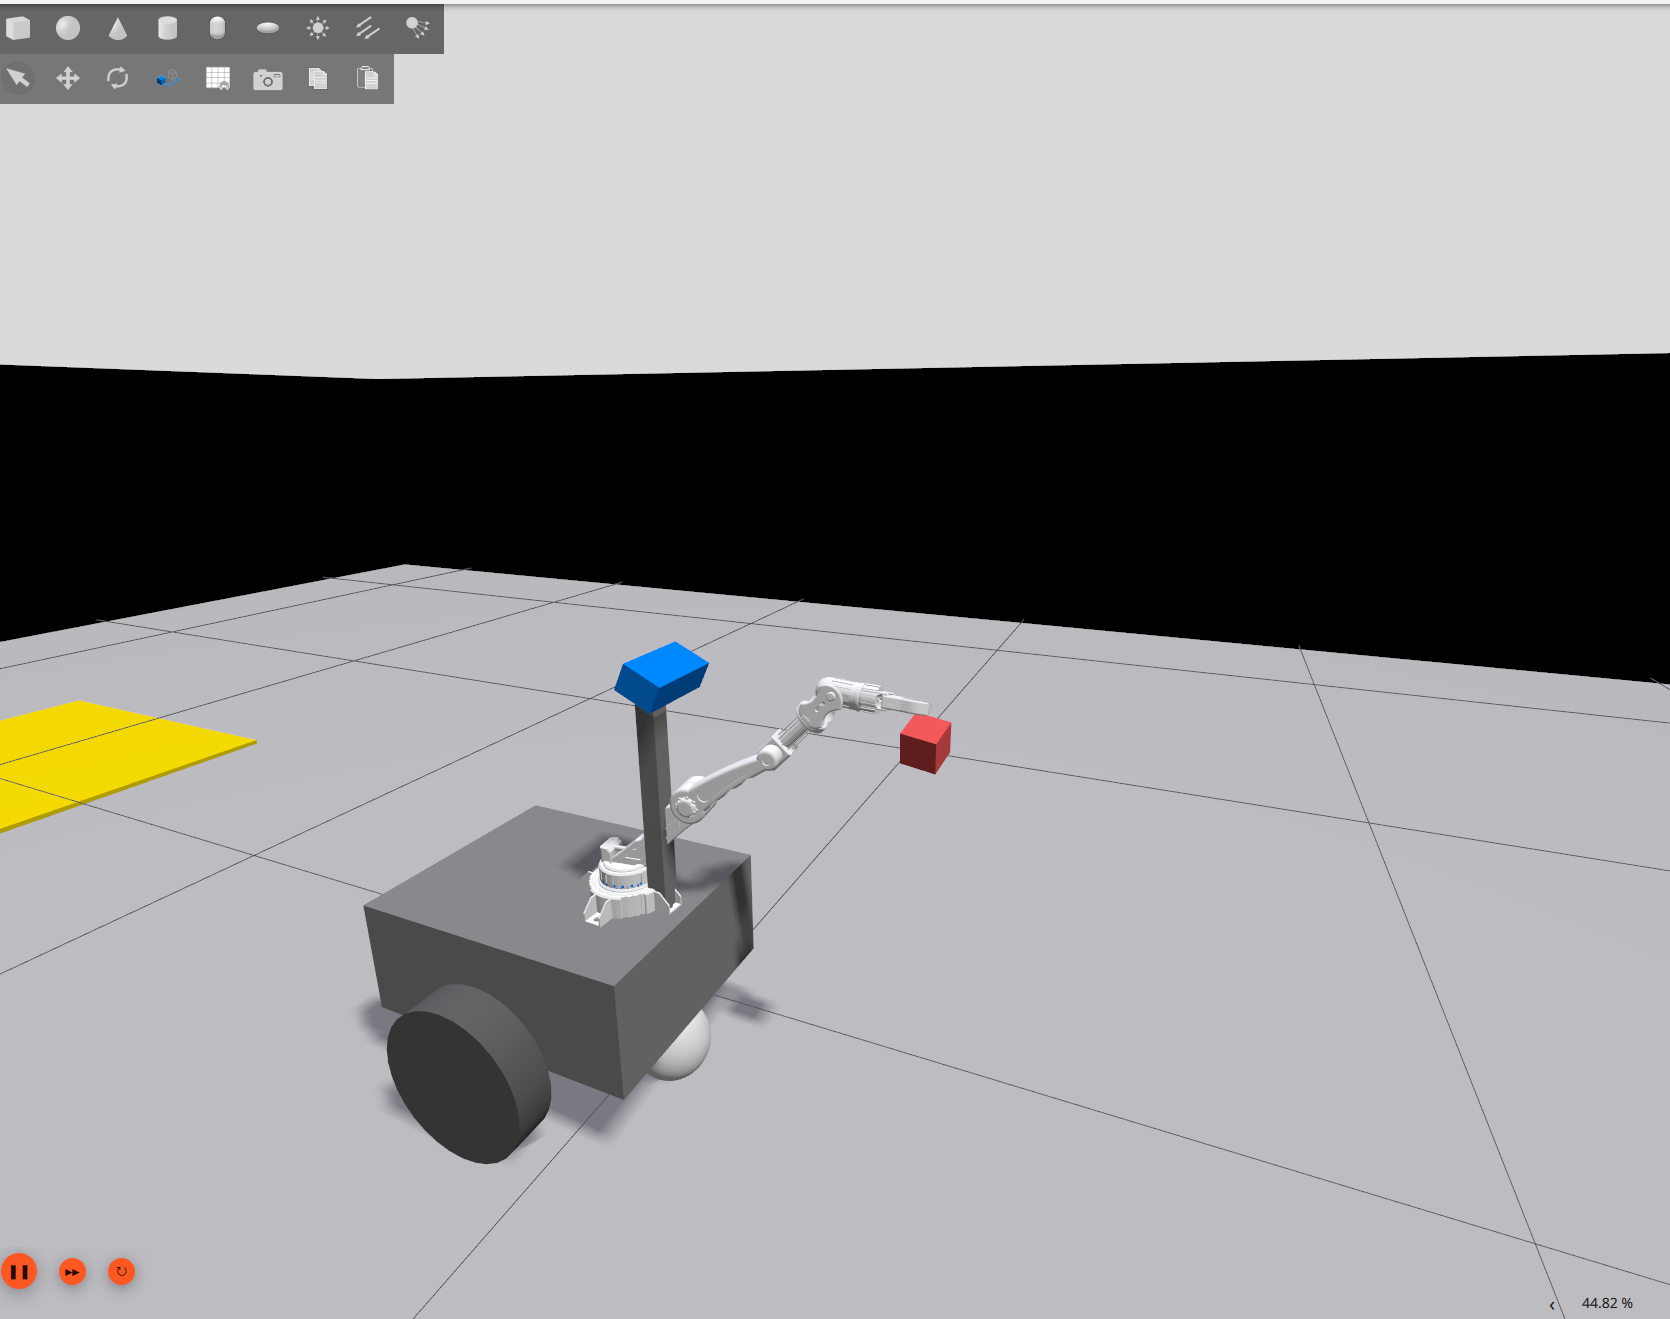
\includegraphics[width=\linewidth]{fig_pick_fail.png}\\[2pt]
  {\small (a) Pick fails: the gripper stops short of the cube}
\end{minipage}\hfill
\begin{minipage}[t]{0.32\textwidth}
  \centering
  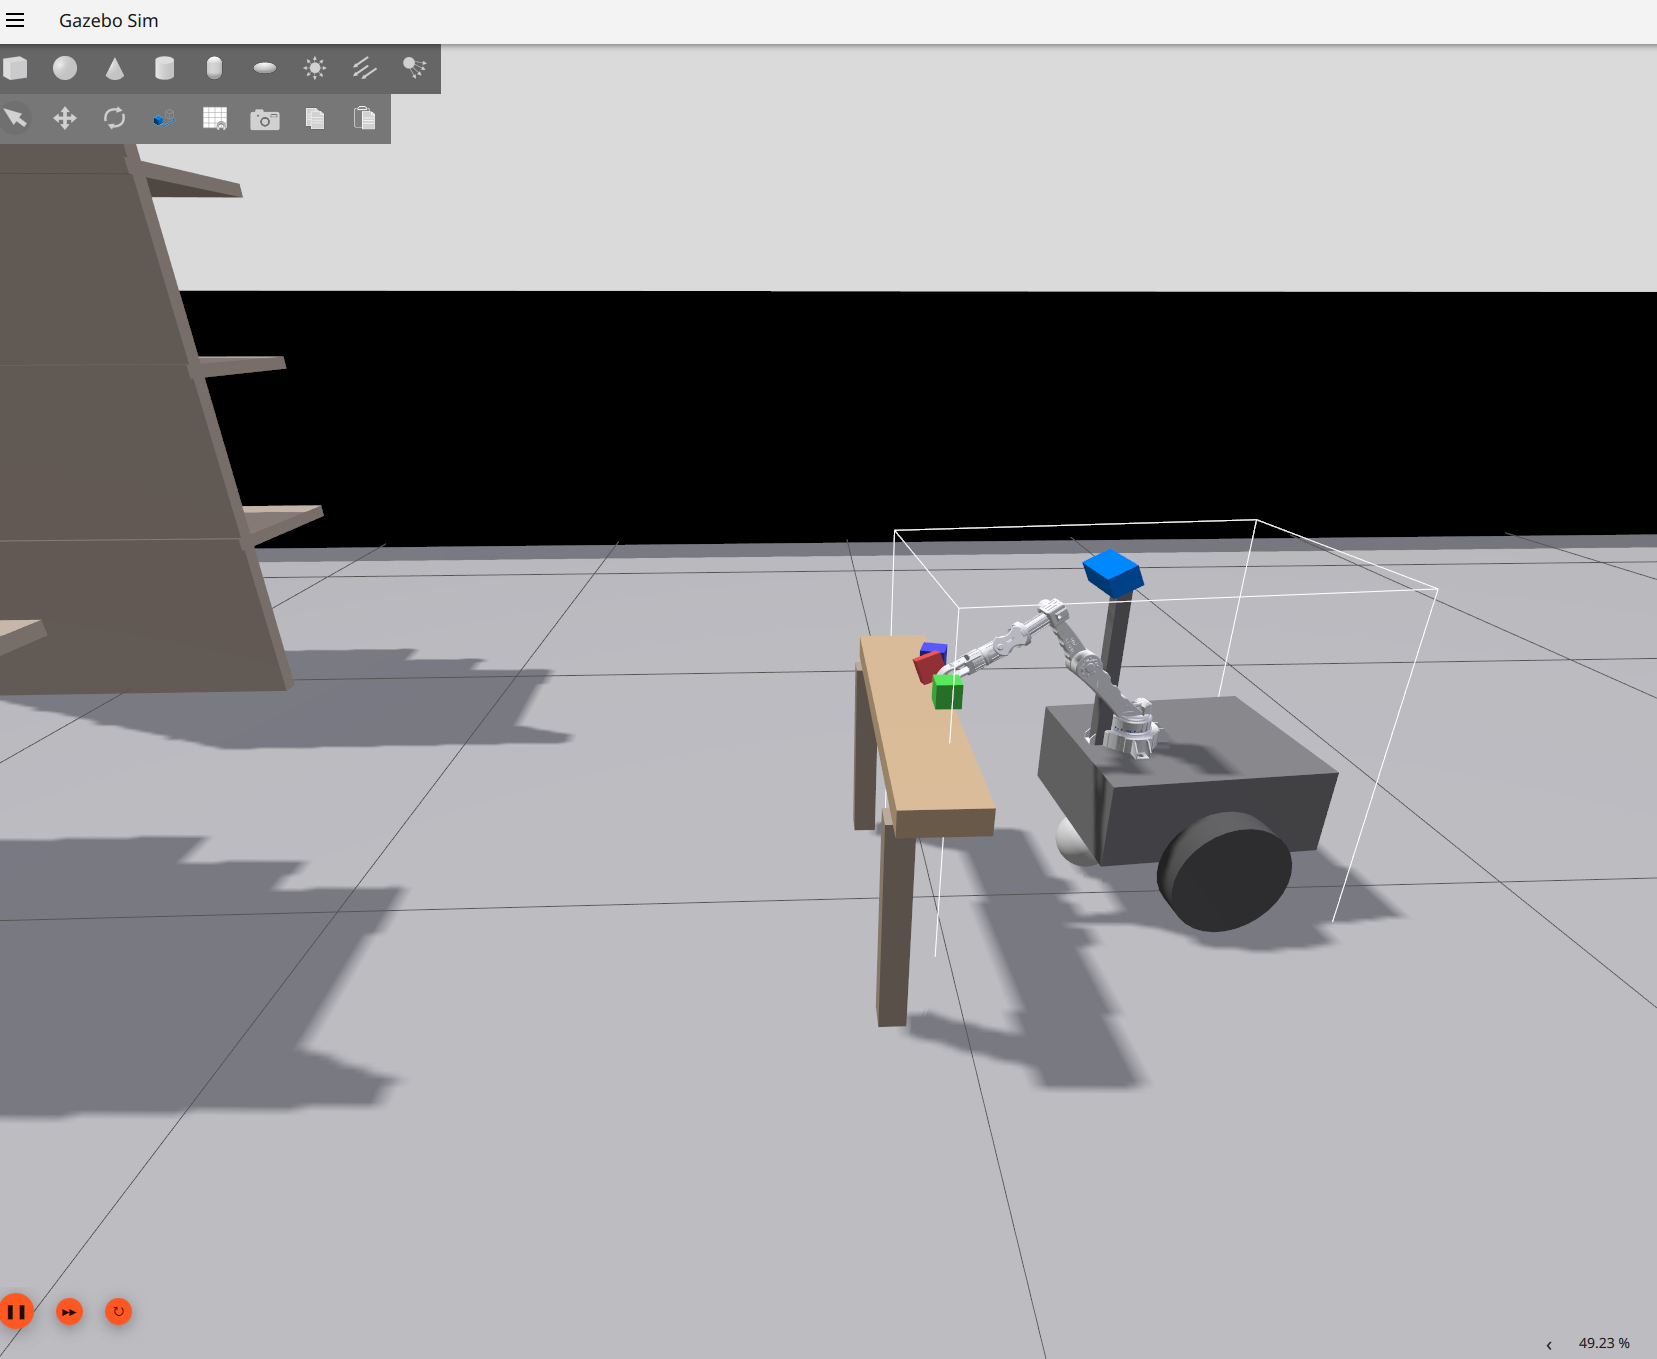
\includegraphics[width=\linewidth]{fig_pick_reach.png}\\[2pt]
  {\small (b) After nudge: arm reaches cube}
\end{minipage}\hfill
\begin{minipage}[t]{0.32\textwidth}
  \centering
  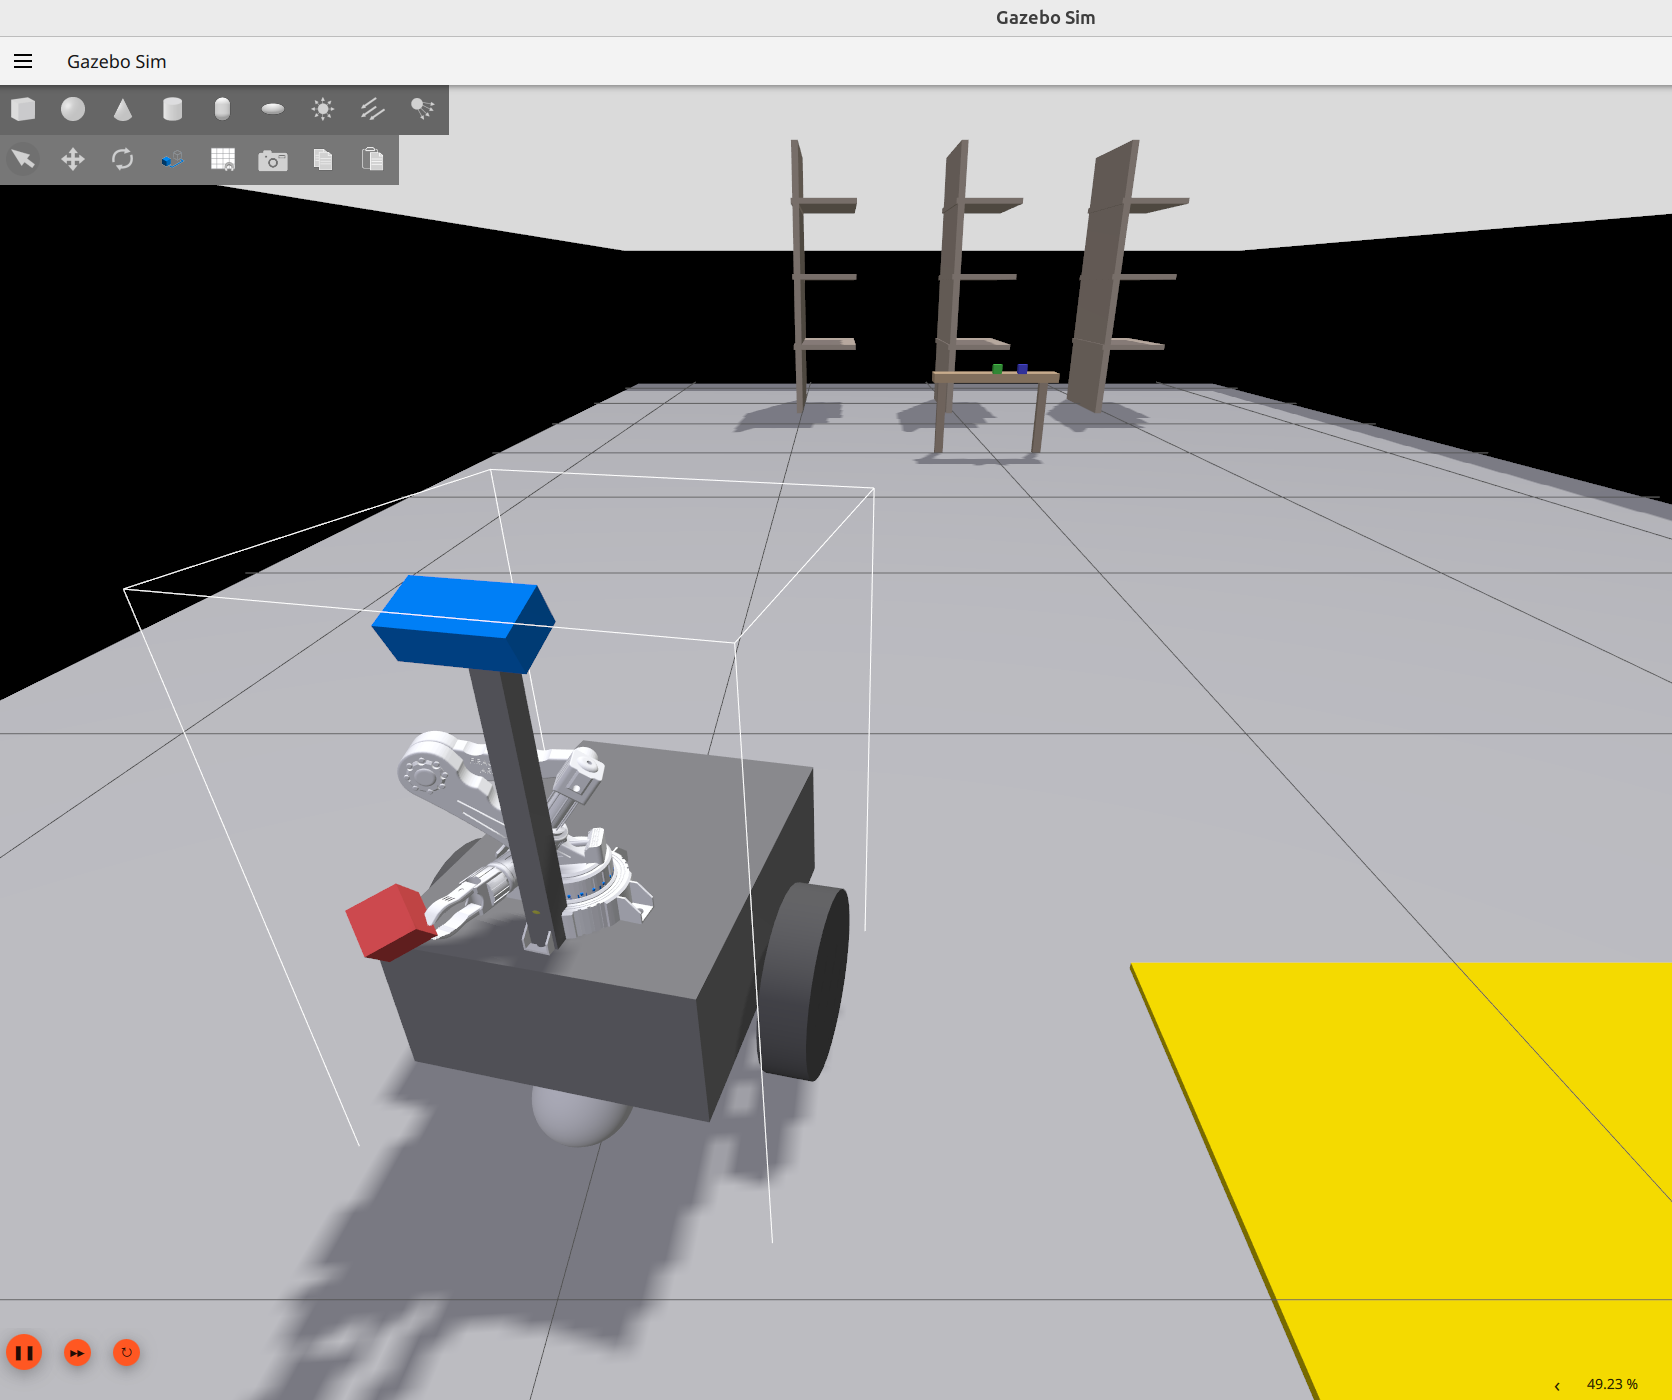
\includegraphics[width=\linewidth]{fig_pick_hold.png}\\[2pt]
  {\small (c) Grasp achieved; cube carried}
\end{minipage}
\caption{Autonomous recovery in S1. A pick attempt fails and the LLM recovers
without scripting: (a)~the pre-grasp pose is unreachable from the navigation
standoff and the gripper stops short of the cube; (b)~after a corrective
forward nudge the arm reaches the cube; (c)~the cube is grasped and carried
toward the dispatch zone. The corrective action is inferred by the LLM from
the tool's failure message. Panel~(a) is taken from a free-space
reachability test rather than a warehouse trial, and is included as an
illustration of the failure geometry only.}
\label{fig:recovery}
\end{figure*}

\subsection{The Deterministic Baseline}

On its calibrated configuration the baseline completed 5/6 single-object
deliveries in 143--249\,s (mean 194\,s, Fig.~\ref{fig:chart}(b)); the
failure was an abort at navigation start. Being perception-blind and branch-free, it is roughly
$2.3\times$ faster than the LLM on average and highly repeatable---but it
cannot react. It succeeds precisely when the world matches the program it
was given, and by construction has no recovery path when it does not. Two
caveats bound what the comparison establishes. The durations are not
measured by the same instrument: the baseline times come from its own
controller and the LLM times from the planner. For scale, the same scripted
task run through the experiment runner's inlined copy---a different
controller whose rates we decline to pool
(Section~\ref{sec:provenance}), cited here only for its
instrumentation---takes 256--507\,s wall-clock including reset overhead. And because the baseline is non-reactive \emph{by construction},
its inability to adapt is a property of how it was written rather than an
experimental finding. We therefore present this contrast as
\emph{determinism versus adaptability} on a shared tool server, and
not as evidence that language models outperform closed-loop alternatives;
Section~\ref{sec:limitations} states the control that would be needed for
the latter.

\subsection{S4: Behaviour Under a Mid-Task Disturbance}
\label{sec:s4}

S4 repeats the S1 delivery, but the runner teleports the red cube to a new
tabletop position 5\,s after \texttt{navigate\_to(table)} is issued---while
the robot is still driving. The displacement is $\approx$18\,cm in $y$,
chosen to stay inside the tabletop's collision bounds (a teleport sets only
the instantaneous pose; physics resumes immediately, so a cube placed past
the edge falls) and away from the far edge, where reachability rather than
replanning would dominate the outcome.

All four frozen-system trials were reported complete, but the mechanism is
not the one the disturbance was designed to probe, and we state that
plainly. The \texttt{pick} tool takes an object label, not coordinates: the
tool server resolves the target from live perception at call time, so the
planner never holds a stale position to be invalidated. In two of the four
runs the post-disturbance \texttt{pick} simply succeeded at the new
location with no corrective action by the planner at all; in the other two
the planner executed the same forward-nudge recovery it uses in S1, in
response to an out-of-reach error rather than to the displacement. No S4
run issued \texttt{detect\_objects}. What S4 demonstrates is that a
perception-resolved action interface absorbs object displacement---an
architectural property, available to any controller built on the same
tools---and not that the language model replans around it.

Two of the four runs are additionally weak as evidence of delivery: the
final \texttt{navigate\_to} and \texttt{place} calls both returned the
planner's 200\,s client-side timeout, after which the model called
\texttt{task\_complete(success=true)} regardless
(Section~\ref{sec:verif}). We therefore report S4 descriptively and draw no
reliability or adaptability claim from it. A disturbance experiment that
would support such a claim needs a target the planner must re-localize
itself, a configuration-matched baseline, and a ground-truth delivery
check; we identify it as the immediate next experiment
(Section~\ref{sec:limitations}).

\subsection{S3: Ordered Multi-Object Sequences}

Across seven two-cube ordered deliveries the planner succeeded in five
(71\%, [36, 92]\%), averaging 19.7 model calls. Four used the phrasing
``move the red cube to dispatch, then the green cube'' and three a more
explicit variant; one of the latter reversed the order---green first, then
red---and was executed in the stated order, which is evidence that the
sequence is read from the command rather than fixed by the tool set. Both
failures terminated at the turn limit after repeated failed tool calls.

Reliability does not survive a third object. On nine trials of ``move all
cubes to the dispatch zone, red one first,'' the planner never completed
the task (0/9, [0, 30]\%), averaging 24.4 model calls; a further five
runner trials of the same command aborted before the planner produced any
call and are excluded. The characteristic trajectory is that the first cube
is delivered, after which repeated navigation and pick failures accumulate
and the planner exhausts its turn budget while trying to recover; longer
runs additionally exposed cumulative localization drift. We report this as
the paper's clearest scalability limitation: the same feedback loop that
supplies recovery on a single object supplies, on a longer horizon, an
unbounded supply of things to recover from.

\subsection{S5: Ambiguous Command Interpretation}

Given ``tidy up the warehouse,'' the LLM correctly interpreted the
ambiguity: it inferred that tidying meant relocating cubes from the table
to the dispatch zone, navigated to the table, and began attempting picks.
Execution then failed: after the approach nudge, a detection cycle
returned no objects, starving the subsequent pick; the planner then
oscillated and incorrectly concluded that the arm's reach was insufficient
(contradicted by S1/S3). The root cause appears to be a perception
field-of-view gap after the local base move, not a reachability wall. S5
thus demonstrates that the LLM \emph{understands} ambiguous instructions
while surfacing a concrete perception-robustness limitation. The baseline
cannot attempt S5 at all, as it performs no language interpretation. With a
single trial this is a case study and not a rate: it shows that one
ambiguous command was resolved into a sensible goal on one occasion, and
supports no generalization about ambiguous-instruction handling.

\subsection{How Success Was Determined, and Its Limits}
\label{sec:verif}

Success in Table~\ref{tab:results} is as reported by the system under test:
for the LLM, its own \texttt{task\_complete(success)} call; for the
baseline, the result of its final step. Neither was checked against the
simulator. Two properties of the stack make this a real limitation rather
than a formality. First, \texttt{place} returns success unconditionally,
including on the fallback path where pre-place IK fails and the object is
released from wherever the arm happens to be. Second, the planner's
per-tool timeout is client-side: when it expires the planner records a
failure while the underlying service call may still be running to
completion, so a timed-out step is genuinely ambiguous rather than
definitely failed.

Auditing the tool traces of the 13 self-reported single-object successes
against their final \texttt{place} call: nine end with \texttt{place}
reporting success; three end with a 200\,s \texttt{place} timeout whose
true outcome is unknown; and one reports ``No object currently held,''
which cannot correspond to a delivery. Read strictly, the single-object
rate is bounded below by 9/16 (56\%) and above by the 13/16 (81\%) we
report, and the S4 row is the most affected, with two of its four runs in
the ambiguous class. We report the upper figure with this bound attached
rather than silently discarding the ambiguous runs.

The release now includes a simulator-side check that reads the cube's true
pose and tests it against the dispatch-zone geometry, recorded as a
separate column alongside the self-reported outcome so that the two can
disagree visibly. It cannot be applied retroactively to the runs reported
here; all future trials in this system are verified by it.

\subsection{Computational Cost of the LLM Planner}

Because the planner queries an LLM at every decision point, its cost is a
practical concern. Table~\ref{tab:cost} summarizes the measured overhead from
the task logs. A single-object delivery averages 8.8 LLM calls at a mean
per-call latency of 1.8\,s, consuming $\approx$42\,k input and $\approx$0.8\,k
output tokens; at Claude Haiku 4.5 list pricing (\$1.00 / \$5.00 per
million input / output tokens) this is \textbf{$\approx$\$0.05 per delivery}.
The two-cube task costs $\approx$\$0.15 per run and the three-cube task
$\approx$\$0.25, scaling with the larger call counts (19.7 and 24.4) and the
longer, re-sent conversation history. Two points follow.
First, the LLM overhead is small relative to the tens-of-seconds cost of
navigation and manipulation---the planner adds seconds of latency, not
minutes. Second, cost grows super-linearly with task length because the
stateless API re-sends the full (uncached) history each turn; prompt caching,
which we did not enable, would substantially reduce the multi-object figure.

\begin{table}[t]
\caption{Measured LLM Planning Overhead (frozen-system runs).}
\label{tab:cost}
\centering
\small
\begin{tabular}{@{}lccc@{}}
\toprule
\textbf{Metric} & \textbf{single} & \textbf{two-cube} & \textbf{three-cube} \\
\midrule
Mean LLM calls / task & 8.8 & 19.7 & 24.4 \\
Mean latency / call & 1.8\,s & 2.0\,s & 2.0\,s \\
Input tokens / task & $\approx$42{,}400 & $\approx$138{,}000 & $\approx$239{,}500 \\
Output tokens / task & $\approx$820 & $\approx$1{,}720 & $\approx$2{,}010 \\
Est.\ API cost / task & $\approx$\$0.047 & $\approx$\$0.147 & $\approx$\$0.250 \\
\bottomrule
\end{tabular}
\end{table}

\subsection{Failure-Mode Summary}

Table~\ref{tab:failures} catalogs the distinct failure modes observed across
all scenarios and separates those resolved during development
(reachability, localization drift) from those that remain on the frozen
system (planner loops, post-nudge perception gaps, tool timeouts). This
separation is the basis for our reporting policy: only the frozen-system
modes count as system performance.

\begin{table}[t]
\caption{Observed Failure Modes.}
\label{tab:failures}
\centering
\small
\begin{tabular}{@{}p{2.2cm}p{2.6cm}p{2.6cm}@{}}
\toprule
\textbf{Mode} & \textbf{Cause} & \textbf{Status} \\
\midrule
Planner loop & LLM oscillates between corrective moves, hits turn limit & Residual; 3/16 single-object, 2/7 two-cube, 9/9 three-cube \\
Perception gap & no detections returned after the approach nudge, starving \texttt{pick} & Residual (frozen); primary S5 failure \\
Reachability & cube at edge of workspace; pre-grasp IK fails & Fixed (0.30\,m approach nudge) \\
Localization drift & grasp-impulse jolt corrupts pose graph over long runs & Mitigated (frozen static map); limits 3-cube runs \\
Timeout & navigation or tool call exceeds its deadline & Residual; 200\,s tool timeout is client-side, leaving 3 reported successes unverified (Sec.~\ref{sec:verif}) \\
\bottomrule
\end{tabular}
\end{table}

% FIGURE 4 -----------------------------------------------------------------
\begin{figure*}[t]
\centering
\pgfplotsset{
  every axis/.append style={
    axis lines=left, line width=0.5pt,
    tick align=outside, tick style={inksecondary, line width=0.4pt},
    label style={font=\footnotesize, text=inksecondary},
    tick label style={font=\scriptsize, text=inksecondary},
    ymajorgrids, grid style={gridgray, line width=0.3pt},
  },
}
\begin{minipage}[t]{0.46\textwidth}
\centering
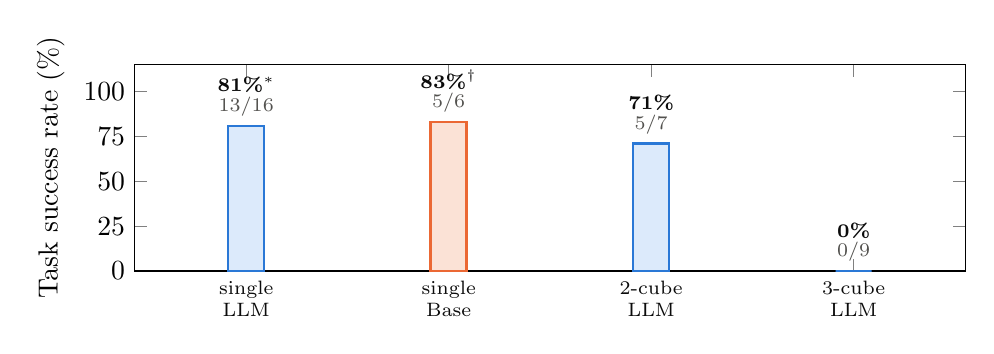
\begin{tikzpicture}
\begin{axis}[
    width=\linewidth, height=4.2cm,
    ymin=0, ymax=115, ytick={0,25,50,75,100},
    ylabel={Task success rate (\%)},
    xmin=0.45, xmax=4.55, xtick={1,2,3,4},
    xticklabels={{single\\LLM}, {single\\Base}, {2-cube\\LLM}, {3-cube\\LLM}},
    x tick label style={align=center, font=\scriptsize, text=inkprimary},
  ]
  \addplot[ybar, bar width=13pt, bar shift=0pt, fill=llmbluefill, draw=llmblue,
           line width=0.9pt] coordinates {(1,81)};
  \addplot[ybar, bar width=13pt, bar shift=0pt, fill=baseorangefill, draw=baseorange,
           line width=0.9pt] coordinates {(2,83)};
  \addplot[ybar, bar width=13pt, bar shift=0pt, fill=llmbluefill, draw=llmblue,
           line width=0.9pt] coordinates {(3,71)};
  \addplot[ybar, bar width=13pt, bar shift=0pt, fill=llmbluefill, draw=llmblue,
           line width=0.9pt] coordinates {(4,0)};
  \node[above, align=center, font=\scriptsize, text=inkprimary] at (axis cs:1,81)
        {\textbf{81\%}$^{\ast}$\\[-1pt]{\scriptsize\color{inksecondary}13/16}};
  \node[above, align=center, font=\scriptsize, text=inkprimary] at (axis cs:2,83)
        {\textbf{83\%}$^{\dagger}$\\[-1pt]{\scriptsize\color{inksecondary}5/6}};
  \node[above, align=center, font=\scriptsize, text=inkprimary] at (axis cs:3,71)
        {\textbf{71\%}\\[-1pt]{\scriptsize\color{inksecondary}5/7}};
  \node[above, align=center, font=\scriptsize, text=inkprimary] at (axis cs:4,0)
        {\textbf{0\%}\\[-1pt]{\scriptsize\color{inksecondary}0/9}};
\end{axis}
\end{tikzpicture}\\[1pt]
{\scriptsize (a) Success rate per scenario}
\end{minipage}\hfill
\begin{minipage}[t]{0.46\textwidth}
\centering
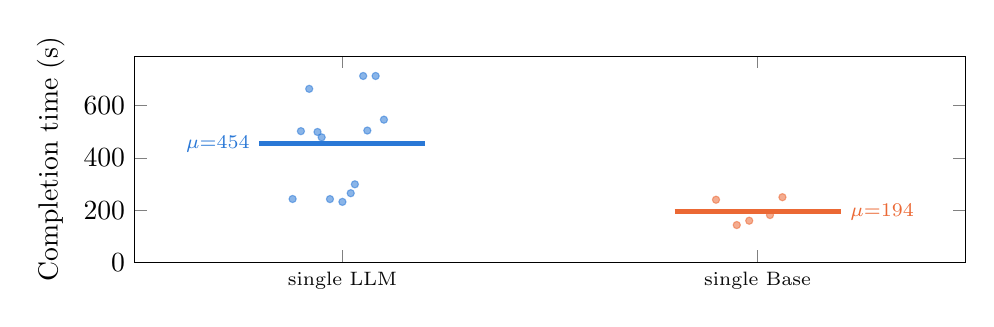
\begin{tikzpicture}
\begin{axis}[
    width=\linewidth, height=4.2cm,
    ymin=0, ymax=790, ytick={0,200,400,600},
    ylabel={Completion time (s)},
    xmin=0.5, xmax=2.5, xtick={1,2},
    xticklabels={{single LLM}, {single Base}},
    x tick label style={font=\scriptsize, text=inkprimary},
  ]
  % individual successful runs (jittered)
  \addplot[only marks, mark=*, mark size=1.3pt, draw=llmblue, fill=llmblue,
           opacity=0.55] coordinates {
    (0.88,242.6) (1.05,713.9) (0.95,478.8) (1.10,546.5) (0.90,502.5)
    (1.03,298.8) (0.97,242.2) (1.08,713.9) (0.92,664.6) (1.00,231.5)
    (1.06,504.8) (0.94,499.4) (1.02,264.7)};
  \addplot[only marks, mark=*, mark size=1.3pt, draw=baseorange, fill=baseorange,
           opacity=0.55] coordinates {
    (1.90,239.7) (2.06,249.4) (1.95,142.7) (2.03,181.0) (1.98,159.3)};
  % mean markers
  \addplot[llmblue, line width=1.7pt] coordinates {(0.80,454)(1.20,454)};
  \addplot[baseorange, line width=1.7pt] coordinates {(1.80,194)(2.20,194)};
  \node[left, font=\scriptsize, text=llmblue] at (axis cs:0.80,454) {$\mu$=454};
  \node[right, font=\scriptsize, text=baseorange] at (axis cs:2.20,194) {$\mu$=194};
\end{axis}
\end{tikzpicture}\\[1pt]
{\scriptsize (b) Completion time, successful runs ($\mu$ = mean)}
\end{minipage}
\caption{Frozen-system comparison (LLM blue, baseline orange).
(a)~Success rate. $^{\ast}$Self-reported; strictly bounded to $[9/16,
13/16]$ (Sec.~\ref{sec:verif}). $^{\dagger}$Baseline on its calibrated
configuration; it is not run on the two- and three-cube commands, which it
cannot parse. (b)~Completion time per successful single-cube run (dots) and
means, measured by each system's own logger: the baseline is faster and
repeatable but rigid; the LLM is slower and more variable because it
perceives, decides, and recovers online.}
\label{fig:chart}
\end{figure*}

% =========================================================================
\section{Discussion: Simulation--Robotics Integration Lessons}
\label{sec:lessons}

Much of the engineering effort---and, we argue, much of the transferable
value of this study---lay in physical-interaction bugs that a pure
planning study would never surface:

\begin{itemize}
\item \textbf{Unsigned reverse distance.} The post-pick reverse maneuver
  (\texttt{drive\_back}, the tool server's internal helper, not the
  \texttt{drive\_distance} tool exposed to the planner)
measured progress as $\sqrt{dx^2 + dy^2}$, which is always positive. With
the arm extended, its inertia could drag the base \emph{forward}, yet this
was counted as backward progress, parking the robot against the table. The
fix is a signed projection onto the commanded backward heading.
\item \textbf{Reach margin dominates reliability.} A 0.15\,m approach
nudge was insufficient for pre-grasp IK; 0.30\,m was required. A single
workspace-geometry constant governed overall single-object success more
than any planning parameter.
\item \textbf{Grasp impulse corrupts localization.} The kinematic-attach
impulse jolted the chassis, injecting phantom LiDAR returns and corrupting
the live SLAM pose graph---the map visibly warped during runs. We
therefore froze the map (static occupancy grid, identity
$map \rightarrow odom$) for experiments, which in turn means our results
exclude real localization drift; we revisit this in
Section~\ref{sec:limitations}. Wheel-joint damping ($damping = 2.0$,
$friction = 0.5$) reduced impulse-induced passive wheel spin.
\item \textbf{Ordering and physics interact.} Reversing with the arm
extended dragged the base off course; homing the arm first (at reduced
velocity) fixed it. A gripper joint oscillated at its limit until velocity
scaling was halved.
\item \textbf{CAD-export correction.} The SolidWorks URDF exporter placed
the kinematic root $\sim$1.7\,m from the assembly origin with an
$8.1^{\circ}$ base tilt baked into the mesh. Bounding boxes do not reveal
face orientation; a PCA plane fit on the base plate's bottom-face
vertices, followed by a Rodrigues correction rotation, was required to
level the robot.
\item \textbf{Framework foot-guns.} Subclassing the \texttt{rclpy} Node
and shadowing its internal \texttt{\_clients} attribute crashed the
planner; navigation to the far zone exceeded a default service timeout and
required raising it to 300\,s.
\end{itemize}

\subsection{A Control-Systems Perspective}
\label{sec:control}

Read through a control lens, the system is a \emph{hierarchical hybrid
dynamical system}: a discrete-event supervisory controller (the LLM) closes
an outer loop around continuous inner loops---Nav2's MPPI controller on the
base, MoveIt/OMPL trajectory tracking on the arm---with the scene state as
sampled feedback and each tool call as a discrete control input.

In these terms, the planner-vs-baseline contrast is the classic
\emph{feedback vs.\ feedforward} distinction. The baseline plays out a fixed reference sequence open-loop:
fast and repeatable, but with no disturbance rejection, so any model--world
mismatch propagates uncorrected. The LLM outer loop is feedback---it
measures the post-action state and corrects, which is why it recovers from
the failed first grasp---and it pays feedback's usual price of added
latency and higher variance (Fig.~\ref{fig:chart}(b)). The residual
planner-loop failure is likewise a \emph{limit cycle} (chattering) in the
decision layer: repeated switching near a decision boundary without
convergence. The hint injected after two identical failures acts as a
coarse \emph{hysteresis / dwell-time} guard; a principled version
(hysteresis switching, or a cost penalty on recently repeated actions) is
the natural route to better convergence. The unsigned \texttt{drive\_back}
bug was a loss of negative feedback: the magnitude $\sqrt{dx^2+dy^2}$
discarded direction, feeding the arm-inertia disturbance back with the
wrong sign until the signed projection restored it.

Two further lessons are disturbance-rejection and conditioning issues. The
grasp attachment is an \emph{impulsive} input coupling through the base
into the localization estimator; wheel-joint damping (higher mechanical
impedance) and the frozen map (estimator decoupling) suppress it. And the
0.30\,m approach nudge is a \emph{kinematic-conditioning margin}: at the
navigation standoff the target sits where the arm Jacobian is poorly
conditioned and IK solutions vanish, and a small base translation restores
manipulability. This view explains why the architecture that grants
adaptability (feedback) also introduces its characteristic failure (limit
cycles); it points to hysteresis/dwell-time switching, disturbance
decoupling, and manipulability-aware base placement as remedies; and it
sets expectations for hardware transfer---contact dynamics, wheel slip, and
odometry drift will re-enter the loop and must be rejected by the inner
controllers, not the LLM.

% =========================================================================
\section{Limitations and Threats to Validity}
\label{sec:limitations}

\textbf{No real-robot validation.} This is a proof-of-concept study
conducted \emph{entirely in simulation}; none of the results have been
reproduced on physical hardware, and we make no claim of sim-to-real
transfer. In particular, grasping is modeled by a proximity-gated
\emph{kinematic attachment} (a DetachableJoint created when the gripper is
within 0.08\,m of the target): it captures whether the arm reaches the object
but \emph{does not validate contact dynamics}---finger--object friction,
grasp-force closure, slip, or compliance. A pick that ``succeeds'' here would
not necessarily succeed on a real gripper. Physical grasp/contact robustness,
sensor noise, actuator dynamics, and real localization drift are therefore
untested and are the primary threats to external validity.

\textbf{Small samples.} Sample sizes are small---the largest single
scenario is $N=9$---so all success rates carry wide confidence intervals
(Table~\ref{tab:results}) and should be read as preliminary. The ambiguous
command was run once and is a case study, not a rate. We evaluate a single
LLM (Claude Haiku 4.5) and do not compare across models or prompts,
although the planner's provider-agnostic client would support it.

\textbf{Unverified outcomes.} Trial success was self-reported by the system
under test rather than checked against the simulator, and four of the
thirteen single-object successes end with a failed or timed-out
\texttt{place} (Section~\ref{sec:verif}). The release now performs a
ground-truth pose check, but it cannot be applied to the runs reported
here.

\textbf{No reactive baseline.} This is the most important open comparison.
Our baseline is perception-blind and non-reactive \emph{by construction},
so its inability to adapt is established by how it was written rather than
measured. The dominant recovery we report---moving forward after an
explicit out-of-reach error---could be encoded as a conventional rule, and
a finite-state machine or behavior tree with access to the same
observations, failure messages, and tools would plausibly match the planner
on the single-object task. What such a control would test, and this paper
does not, is whether language-model planning offers an advantage over
simpler closed-loop methods rather than over open-loop ones. We regard it
as the necessary next experiment, together with a disturbance scenario in
which the planner must re-localize the target itself.

\textbf{Simplified environment.} The frozen static map removes the
localization drift a deployed system would face---and which our longer
development runs began to expose---motivating tighter sensor fusion and
periodic relocalization as future work. Objects are primitive uniformly
coloured cubes detected by colour segmentation, not cluttered real-world
items. Finally, baseline and LLM success rates are measured over different
denominators, on differently tuned configurations, and with wall-clock
durations taken from different loggers; we therefore compare them
qualitatively (determinism vs.\ adaptability) rather than as a single
head-to-head percentage.

% =========================================================================
\section{Conclusion}

A general-purpose LLM, constrained to a fixed tool interface and closed
with a structured scene state after every action, can drive a complete
ROS~2 mobile-manipulation stack from a natural-language sentence
and---critically---recover autonomously from realistic execution failures,
reporting 81\% of single-object deliveries complete (strictly, between 9/16
and 13/16) where a hardcoded baseline is fast but rigid. Reliability
degrades sharply with sequence length---71\% on two cubes, zero on
three---and under ambiguous commands whose execution stresses perception,
and we report these limits alongside the successes. We are careful about
what the comparison establishes: the baseline is non-reactive by
construction, so these results show that an LLM can select a sensible
correction from a general tool interface, not that it outperforms a
reactive controller given the same observations. We believe the failure
catalogue and the concrete integration lessons are as valuable to
practitioners as the headline success rate. Future work is accordingly
specific: a reactive non-LLM baseline (finite-state machine or behavior
tree) with access to the same tools and failure messages, a disturbance
experiment with ground-truth delivery checking, cross-model comparison,
and real-robot transfer.

\section*{Reproducibility}
All packages, tool schemas, the LLM system prompt, the world file, and the
experiment/logging code are available in the project repository:
\url{https://github.com/Firaol-Tes/aset_ws}.

% =========================================================================
\begin{thebibliography}{99}

\bibitem{saycan}
M.~Ahn \emph{et~al.}, ``Do as {I} can, not as {I} say: Grounding language
in robotic affordances,'' in \emph{Proc. Conf. Robot Learning (CoRL)},
2022, arXiv:2204.01691.
\bibitem{codeaspolicies}
J.~Liang \emph{et~al.}, ``Code as policies: Language model programs for
embodied control,'' in \emph{Proc. IEEE Int. Conf. Robotics and
Automation (ICRA)}, 2023.
\bibitem{progprompt}
I.~Singh \emph{et~al.}, ``{ProgPrompt}: Generating situated robot task
plans using large language models,'' in \emph{Proc. IEEE Int. Conf.
Robotics and Automation (ICRA)}, 2023.
\bibitem{palme}
D.~Driess \emph{et~al.}, ``{PaLM-E}: An embodied multimodal language
model,'' in \emph{Proc. Int. Conf. Machine Learning (ICML)}, 2023.
\bibitem{rt2}
A.~Brohan \emph{et~al.}, ``{RT-2}: Vision-language-action models transfer
web knowledge to robotic control,'' in \emph{Proc. Conf. Robot Learning
(CoRL)}, 2023.
\bibitem{voxposer}
W.~Huang \emph{et~al.}, ``{VoxPoser}: Composable {3D} value maps for robotic
manipulation with language models,'' in \emph{Proc. Conf. Robot Learning
(CoRL)}, 2023.
\bibitem{llmrobosurvey}
F.~Zeng, W.~Gan, Y.~Wang, N.~Liu, and P.~S.~Yu, ``Large language models for
robotics: A survey,'' \emph{arXiv preprint} arXiv:2311.07226, 2023.
\bibitem{react}
S.~Yao \emph{et~al.}, ``{ReAct}: Synergizing reasoning and acting in
language models,'' in \emph{Proc. Int. Conf. Learning Representations
(ICLR)}, 2023.
\bibitem{toolformer}
T.~Schick \emph{et~al.}, ``{Toolformer}: Language models can teach
themselves to use tools,'' in \emph{Advances in Neural Information
Processing Systems (NeurIPS)}, 2023.
\bibitem{innermonologue}
W.~Huang \emph{et~al.}, ``Inner monologue: Embodied reasoning through
planning with language models,'' in \emph{Proc. Conf. Robot Learning
(CoRL)}, 2022.
\bibitem{chatgptrobotics}
S.~Vemprala, R.~Bonatti, A.~Bucker, and A.~Kapoor, ``{ChatGPT} for
robotics: Design principles and model abilities,'' \emph{IEEE Access},
2024.
\bibitem{ros2}
S.~Macenski, T.~Foote, B.~Gerkey, C.~Lalancette, and W.~Woodall, ``Robot
operating system 2: Design, architecture, and uses in the wild,''
\emph{Science Robotics}, vol.~7, no.~66, 2022.
\bibitem{nav2}
S.~Macenski, F.~Mart\'in, R.~White, and J.~Ginés~Clavero, ``The marathon
2: A navigation system,'' in \emph{Proc. IEEE/RSJ Int. Conf. Intelligent
Robots and Systems (IROS)}, 2020.
\bibitem{moveit}
D.~Coleman, I.~\c{S}ucan, S.~Chitta, and N.~Correll, ``Reducing the
barrier to entry of complex robotic software: A {MoveIt!} case study,''
\emph{J. Software Engineering for Robotics}, 2014.
\bibitem{yolov8}
G.~Jocher, A.~Chaurasia, and J.~Qiu, ``Ultralytics {YOLOv8},'' 2023.
[Online]. Available: \url{https://github.com/ultralytics/ultralytics}
\end{thebibliography}

\end{document}
